
%% bare_conf.tex
%% V1.4b
%% 2015/08/26
%% by Michael Shell
%% See:
%% http://www.michaelshell.org/
%% for current contact information.
%%
%% This is a skeleton file demonstrating the use of IEEEtran.cls
%% (requires IEEEtran.cls version 1.8b or later) with an IEEE
%% conference paper.
%%
%% Support sites:
%% http://www.michaelshell.org/tex/ieeetran/
%% http://www.ctan.org/pkg/ieeetran
%% and
%% http://www.ieee.org/

%%*************************************************************************
%% Legal Notice:
%% This code is offered as-is without any warranty either expressed or
%% implied; without even the implied warranty of MERCHANTABILITY or
%% FITNESS FOR A PARTICULAR PURPOSE! 
%% User assumes all risk.
%% In no event shall the IEEE or any contributor to this code be liable for
%% any damages or losses, including, but not limited to, incidental,
%% consequential, or any other damages, resulting from the use or misuse
%% of any information contained here.
%%
%% All comments are the opinions of their respective authors and are not
%% necessarily endorsed by the IEEE.
%%
%% This work is distributed under the LaTeX Project Public License (LPPL)
%% ( http://www.latex-project.org/ ) version 1.3, and may be freely used,
%% distributed and modified. A copy of the LPPL, version 1.3, is included
%% in the base LaTeX documentation of all distributions of LaTeX released
%% 2003/12/01 or later.
%% Retain all contribution notices and credits.
%% ** Modified files should be clearly indicated as such, including  **
%% ** renaming them and changing author support contact information. **
%%*************************************************************************


% *** Authors should verify (and, if needed, correct) their LaTeX system  ***
% *** with the testflow diagnostic prior to trusting their LaTeX platform ***
% *** with production work. The IEEE's font choices and paper sizes can   ***
% *** trigger bugs that do not appear when using other class files.       ***                          ***
% The testflow support page is at:
% http://www.michaelshell.org/tex/testflow/



\documentclass[conference]{IEEEtran}


% *** CITATION PACKAGES ***
%
%\usepackage{cite}
% cite.sty was written by Donald Arseneau
% V1.6 and later of IEEEtran pre-defines the format of the cite.sty package
% \cite{} output to follow that of the IEEE. Loading the cite package will
% result in citation numbers being automatically sorted and properly
% "compressed/ranged". e.g., [1], [9], [2], [7], [5], [6] without using
% cite.sty will become [1], [2], [5]--[7], [9] using cite.sty. cite.sty's
% \cite will automatically add leading space, if needed. Use cite.sty's
% noadjust option (cite.sty V3.8 and later) if you want to turn this off
% such as if a citation ever needs to be enclosed in parenthesis.
% cite.sty is already installed on most LaTeX systems. Be sure and use
% version 5.0 (2009-03-20) and later if using hyperref.sty.
% The latest version can be obtained at:
% http://www.ctan.org/pkg/cite
% The documentation is contained in the cite.sty file itself.


% *** GRAPHICS RELATED PACKAGES ***
%
\ifCLASSINFOpdf
   \usepackage[pdftex]{graphicx}
  % declare the path(s) where your graphic files are
   \graphicspath{{pic/}}
  % and their extensions so you won't have to specify these with
  % every instance of \includegraphics
   \DeclareGraphicsExtensions{.png}
\else
  % or other class option (dvipsone, dvipdf, if not using dvips). graphicx
  % will default to the driver specified in the system graphics.cfg if no
  % driver is specified.
  % \usepackage[dvips]{graphicx}
  % declare the path(s) where your graphic files are
  % \graphicspath{{../eps/}}
  % and their extensions so you won't have to specify these with
  % every instance of \includegraphics
  % \DeclareGraphicsExtensions{.eps}
\fi

% correct bad hyphenation here
\hyphenation{op-tical net-works semi-conduc-tor}


\begin{document}
\title{A Tool for Visualizing Patterns of Spreadsheet Function Combinations}


% author names and affiliations
% use a multiple column layout for up to three different
% affiliations
\author{\IEEEauthorblockN{Justin A. Middleton}
\IEEEauthorblockA{North Carolina State University\\
Raleigh, North Carolina}}


% use for special paper notices
%\IEEEspecialpapernotice{(Invited Paper)}




% make the title area
\maketitle

% As a general rule, do not put math, special symbols or citations
% in the abstract
\begin{abstract}
Spreadsheet environments often come equipped with a plethora of functions to manipulate and calculate data, but it can be difficult to understand how end-users employ these functions in practice. Without this knowledge, both researchers and practitioners lack information about how end users construct sophisticated programs from these basic elements. We developed a tool that visualizes patterns of how functions are combined into formulae within Excel spreadsheets. Using the Enron spreadsheet dataset as an example, this paper shows how the tool can display both common and anomalous formulas and their respective contexts in an actual workbook.
\end{abstract}

% no keywords




% For peer review papers, you can put extra information on the cover
% page as needed:
% \ifCLASSOPTIONpeerreview
% \begin{center} \bfseries EDICS Category: 3-BBND \end{center}
% \fi
%
% For peerreview papers, this IEEEtran command inserts a page break and
% creates the second title. It will be ignored for other modes.
\IEEEpeerreviewmaketitle



\section{Introduction}
% no \IEEEPARstart
Business and research alike owe their debts to spreadsheets, the table-based interface which empowers users to organize and manipulate huge bodies of data [citation for definition]. Their allure is in their versatility: while the novice end user can work without a deep knowledge of programming, the expert can expedite their work with a variety of built-in operations, or functions.\footnote{https://support.office.com/en-us/article/Excel-functions-alphabetical-b3944572-255d-4efb-bb96-c6d90033e188} As such, it should be of little surprise when Scaffidi and colleagues estimated that by 2012, over 50 million U.S. workers could be using them, including the 25 million who would be writing programs out of the functions included \cite{scaffidi2005estimating}.\par

Considering this ubiquity, it's crucial to get spreadsheets right. Our failures in their use can be ruinous, as in 2012 when the influential findings on economic growth were reversed by a selection error, among other horror stories.\footnote{http://www.eusprig.org/horror-stories.htm}

Fortunately, the vanguards of spreadsheet research have assembled, organized, and released a number of spreadsheet corpora to inform work on how people actually use these tools in different contexts. Collections like EUSES \cite{fisher2005euses}, FUSE \cite{barik2015fuse}, and the Enron corpus \cite{hermans2015enron} have already enabled fruitful work across the field, such as detecting code smells in spreadsheets \cite{hermans2012detecting} \cite{cunha2012smellsheet}.  \par

A tool, then, which empowers users of many intentions to explore these datasets would be rife with potential. On a simple level, the tool could provide concrete statistics on which functions are used in practice most (or least) often, and what other functions that work in conjunction with them. These numbers, then, could inform future work done on intelligently recommending functions to users or generating new formulas from these patterns of function use. Spreadsheet APIs, likewise, could be augmented or pruned through the discovery of frequent combinations or anomalous use of functions. Furthermore, if the tool maintains the connection between patterns and the actual, it could serve as a boon to educators as well, guiding lesson plans to the most commonly employed functions and offering a bounty of instructive (and real) examples.\par
This paper presents such a tool, informed by such varied sources, that visualizes not how people employ individual Excel functions but how they combine to make more sophisticated spreadsheet formulas. 


\section{Related Work}
This tool comes from a line of spreadsheet visualization tools before it, each with a different focus. Some tools, such as Igarashi and colleague's fluid visualizations \cite{igarashi1998fluid}, seek to visualize the hidden formulas within a spreadsheet by imposing the dataflow graphs over the cells. Likewise, Clermont \cite{clermont2003scalable} (and Hipfl \cite{hipfl2008using}, who extended his work) explored various ways of visualizing groups of related cells through similar functions, neighbors, or references. Others focus on creating visualizations outside of the sheets: Hermans and colleagues address a spreadsheet programmer's information needs through their work on the tools GyroSAT \cite{hermans2011supporting} and Breviz \cite{hermans2011breviz} to make dataflow diagrams of individual spreadsheets. These, however, tend to focus on individual spreadsheets and not bodies of them. \par
Nevertheless, other studies and tools focus more on evaluating the content of the cells therein. (Hermans, Smellsheet) \par
Other studies focus on API and built-in function use outside the domain of spreadsheets. [RESEARCH ON API STUDIES]  

\section{Approach}
\subsection{Goals}
In visualizing the spreadsheet data, I outlined a few core goals for what the tool should accomplish:
\begin{itemize}
	\item [1] \textbf{Draw an interactive interface to explore observed function combinations.} The combination space for all Excel functions is massive, let alone the space for observed formulas. Working from data with actual referents in practice, the tool must aid the user in navigating this space.
	\item [2] \textbf{Emphasize the quantitative patterns in formula construction.} The tool, accommodating datasets of a few spreadsheets to millions, should address the questions of how often the end users employed a certain function and where they used it. In this way, it must show precise metrics, such as frequency of  use and depth of function nesting, of the dataset it conveys.
	\item [3] \textbf{Promote a qualitative understanding of the patterns.} Lest these patterns remain abstract, the tool should supplement its observations with concrete instances of relevant formulas from the corpus. Ideally, it should even direct users to the exact cell in the spreadsheets where the formula was used, contextualizing the functions. 
\end{itemize} \par
Likewise, to bound our scope, we outlined a few goals to specifically avoid accomplishing with this:
\begin{itemize}
	\item [!1] \textbf{Do not try to directly explain what a function does.} Though the tool tries to foster tries understanding by linking pattern to example, it won't provide a precise description of what a function accomplishes. The tool's user must infer this.
	\item [!2] \textbf{Do not create new formulas.} This is essentially an exploratory tool, not a generative one. It should not produce any information other than new views of the original data. 
	%TODO: I do have an idea which could actually do the below, but, eh, it would take
	%TODO: a fair amount of time to implement.
	\item [!3] \textbf{Do not visualize individual formulas.} Though there is room to explore the place of a single function in the group, the tool must design the core visualization around the entire body of data, not the other way around.
\end{itemize}

\subsection{Description}
To show how this all came together and demonstrate the interface, we will use an example of a quick task: discovering what kind of conditions people use in IF statements. Considering only formulas in which the IF function itself is the top-level function (that is, not nested within another function), we will approach a tree that begins like this:
 
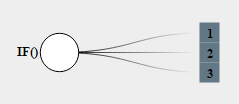
\includegraphics{start}

The visualization so far comprises two types of node: the circle, which represents a discrete function in the formula and is size according to its relative frequency (the top-level node, by definition, will be the largest); and the numbered squares, which represent the positions of arguments within its parent function. From this, we can infer that, of the times it was observed, IF can have at most three arguments passed into it, which corresponds with its specifications in the API.\footnote{https://support.office.com/en-us/article/IF-function-69aed7c9-4e8a-4755-a9bc-aa8bbff73be2} \par
Knowing that it is the first argument which contains the conditionals, we click on the square labeled "1" to explore. To save space, when more than 10 unique arguments have been observed in any position, the tool displays only the first ten, with an option to display the rest. The results are shown below:

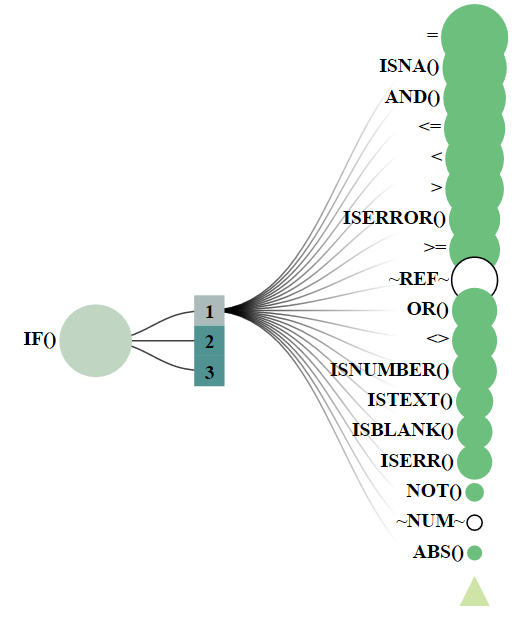
\includegraphics[width=.43\textwidth]{IFexpand}

As expected, we see that IF contains as its first argument a number of comparison operators, such as = and <=, and boolean-returning functions, like ISNA and AND, with simple equality being the most common and some use as ABS being the least seen of everything actually used.
From here, we can further explore the common options among these functions. Clicking on the "=" node will yield two arguments, it being a binary operator, and expanding each of them will peer into the range of common values of equality comparison:

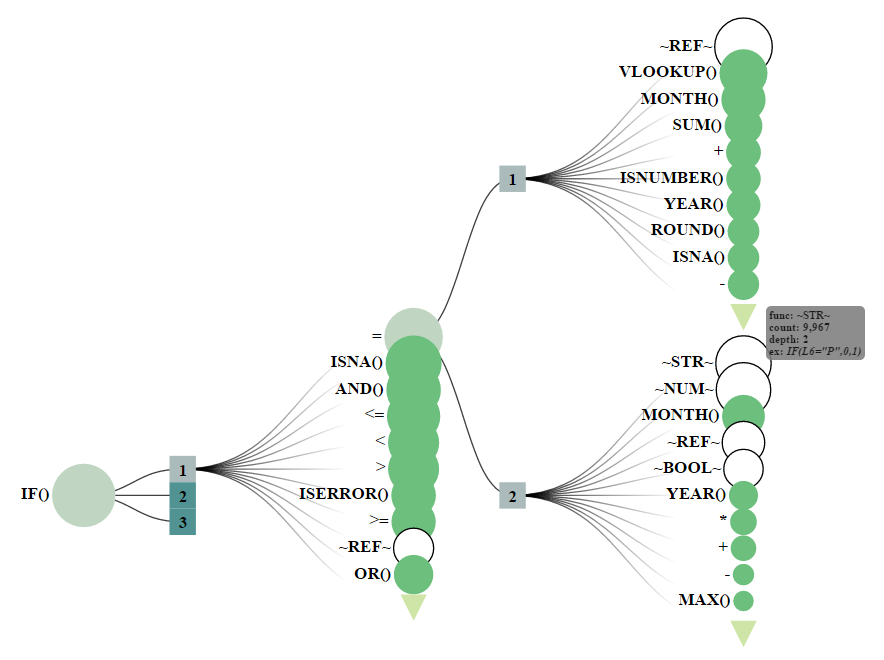
\includegraphics[width = .43\textwidth]{IFargslabel}

For both sides of the equal sign, the operator has certain types of arguments which predominate over the others: on the left side is most often a reference to another cell; on the right, a string or number literal, which makes sense for the case of confirming a value in another cell before assigning this one. Furthermore, if the concept is difficult to imagine is practice, a tooltip accompanies each function node in the tree, providing a concrete example of a function that uses this structure and where it can be found.

\subsection{Design}
Early in the process, we decided that the tree form would be a suitable fit to represent the parent-child or caller-callee relationships inherent in the data, given the composition of formulas as functions and their arguments (which could be yet more functions). By adapting this structure to accommodate a broad range of possibilities for nested functions, the branching factor depends on both the number of arguments in a function and the number of possible functions observed as an argument in a function. \par
Guided by the goals in section A, we faced a number of decision points, which we describe below, before we arrived at the design shown above.


\begin{itemize}
	\item [1a] \textit{Copied formulas}: Excel allows users to spread a formula over an area, repeating the same task in each cell with minor adjustments. Without checking for this, the analysis may not reveal the functions most commonly used together but rather the formulas most often applied to large areas. To combat this, we converted formulas from their native A1 format to the relative R1C1, in which copied formulas should be identical, and reduced the records to unique R1C1 formulas per sheet.
	\item [1b] \textit{Optional arguments}: How should the tool handle functions which accept a variable number of arguments? SUM, for example, can have anywhere from 1 to 255, and IF can accept either 2 or 3. \footnote{https://support.office.com/en-us/article/Excel-functions-by-category-5f91f4e9-7b42-46d2-9bd1-63f26a86c0eb} Without prior evidence, it's possible that spreadsheet programmers use different techniques for different numbers arguments. To account for this, we separate and analyze the different quantities of arguments observed for each function; the tool, however, uses as default all of the options collapsed into a single representation.
\end{itemize}

\begin{itemize}
	%TODO: A picture would go well here.
	\item [2a] \textit{Importance of depth}: When a function appears within another, should it be analyzed only as a nested function or would it also be valid to analyze the nested function on its own? If the former, then information about the same function will be scattered across different trees with no way to aggregate them. If the latter, then the tool will analyze some functions multiple times to capture every possible level of nesting. Both approaches have benefits and drawbacks, and so we included both.
	\item [2b] \textit{Pattern density}: How should the tool quantitatively order its elements: by a function's raw frequency or by the unity of patterns it leads to? For example, if SUM has for its first argument two possibilities, one which itself contains 1000 unique argument possibilities with 1 occurrence each (high frequency, low pattern density) and another seen with 2 argument possibilities of 100 occurrences each (low frequency, high pattern density), which would be more interesting to emphasize? The answer depends on the nuances of the questions, but for simplicity, I've shown the former.
	\item [2c] \textit{Non-functions}: How should the tool represent everything in the formula that isn't a function: numbers, string literals, errors, references, etc? Since these don't accept arguments, they will adorn the tree as leaves, and their precise content won't affect the functions around them as long as their types are known. As such, in the visualization, all of these nodes are replaced and aggregated under their types.
\end{itemize}

\begin{itemize}
	\item [3a] \textit{Suitable examples}: Goal 3 supports the inclusion of examples in the visualization as a way of tying pattern to example, but how should examples be chosen? For this, the simpler is the better, and we made the broad working assumption that shorter (by character length) functions are simpler, and thus chose the shortest available.
	\item [3b] \textit{Spreadsheet connections}: Is it possible to contextualize these examples even better? Yes, by leading the user directly back to the originating spreadsheet. The tool hyperlinks each example, then, back to the file that contains it, providing sheet, row, and column numbers if it doesn't open directly there.
\end{itemize}



\subsection{Implementation}
We can view the final visualization as the product of two discrete processes:
\begin{itemize}
	\item \textit{Collection}: Given a set of Excel sheets, the tool, written mostly in Java, uses Apache POI\footnote{https://poi.apache.org/} to identify and iterate over every cell containing a valid formula. Afterward, it calls POI's formula parser to break the formula text into an ordered set of individual tokens, which the tool then parses into the tree-like form by which it is recorded. When all formulas have been analyzed like this, it produces JSON files for each top-level function in the set.
	\item \textit{Presentation}: The JSON files, meanwhile, feed into the presentation code, implemented in Javascript with much help from the visualization library D3\footnote{https://d3js.org/}. 
\end{itemize}
When the presentation code displays the tree, it shows two types of nodes with different meanings: the circles represent a function that has been observed at that structural place, and hovering over these yields a tooltip with supplementary information and examples; and squares, which represent the argument positions for the function which is their parent. For example, if the IF function has been observed with three arguments, 3 squares will extend from it as children. Clicking on the square labeled '1' will yield more circles, all of which are functions or values that the tool observed as the first argument in an IF function; clicking on '2' will yield those possibilities in the second position; and so on.



\subsection{Limitations}
Because the data collection depends on POI's formula parser, it affords no leeway or partial information from a formula; it either processes it perfectly or throws it out. As such, the visualization inhibits insight into anything with syntactical errors or third-party functions that can't be evaluated without additional tools. Note, however, that this does not include standard Excel errors like \#REF! and \#DIV/0, which the parser handles well. \par
Many functions have an expected order of arguments, but some, like SUM and MATCH, can be reordered in various ways and maintain their value. However, the representation that this tool uses reinforces for all functions that the order is important, even in these exceptions. \par
A larger and related problem is the loss of argument combination. In the example in section B, we saw how the tools conveys which arguments are used most often on each side of an equals sign, but it does not encode how these whether references were actually compared to strings and numbers the most or whether it corresponded more to all the arguments beneath those two 

\section{Case Study}

[to be filled in]

\section{Conclusion}

[to be filled in]

-extensible to other spreadsheets?
% conference papers do not normally have an appendix


% use section* for acknowledgment
\section*{Acknowledgment}
This material is based upon work supported in whole or in part with funding from the Laboratory for Analytic Sciences (LAS). Any opinions, findings, conclusions, or recommendations expressed in this material are those of the author(s) and do not necessarily reflect the views of the LAS and/or any agency or entity of the United States Government.

% references section

% can use a bibliography generated by BibTeX as a .bbl file
% BibTeX documentation can be easily obtained at:
% http://mirror.ctan.org/biblio/bibtex/contrib/doc/
% The IEEEtran BibTeX style support page is at:
% http://www.michaelshell.org/tex/ieeetran/bibtex/
\bibliographystyle{IEEEtran}
% argument is your BibTeX string definitions and bibliography database(s)
\bibliography{paper}
%
% <OR> manually copy in the resultant .bbl file
% set second argument of \begin to the number of references
% (used to reserve space for the reference number labels box)
%\begin{thebibliography}{1}
%
%\bibitem{IEEEhowto:kopka}
%H.~Kopka and P.~W. Daly, \emph{A Guide to \LaTeX}, 3rd~ed.\hskip 1em plus
%  0.5em minus 0.4em\relax Harlow, England: Addison-Wesley, 1999.
%
%
%\end{thebibliography}




% that's all folks
\end{document}


